% arara: pdflatex
% arara: biber
% arara: makeindex
% arara: nomencl
% arara: pdflatex
% arara: pdflatex

\documentclass[a4paper,12pt]{article}
%\RequirePackage[l2tabu,orthodox]{nag}

\usepackage{upreport}
\usepackage{tabularx}
\usepackage{amssymb}
\addbibresource{report.bib}
\title{Noob's Guide to \LaTeX}
\subject{CSC 421}
\date{\today}

%Nomenclature unit command
\newcommand{\nomunit}[1]{%
\renewcommand{\nomentryend}{\hspace*{\fill}#1}}

% Create a custom user command or run the following 
%  makeindex %.nlo -s nomencl.ist -o %.nls
% execute this command after compiling your file once, then compile a second time to generate a nomenclature table



\begin{document}
\maketitle
\makecoverpage

\pagestyle{plain}
\thispagestyle{plain}
\pagenumbering{roman}

\begin{center}
\LARGE\textbf{\thetitle}
\end{center}

\section*{Synopsis}
\addcontentsline{toc}{section}{Synopysis}%
Welcome to the Noob's guide.
This section has only been included for reference on how to use it when comparing the source code to the resulting document.
Please continue to the Introduction, Section~\ref{sec:Introduction}.
\setcounter{page}{3}

\newpage
\tableofcontents

\iftotalfigures%
\newpage%
\listoffigures%
\fi

\iftotaltables%
\newpage%
\listoftables%
\fi

\newpage

%\chapter*{Nomenclature}
\printnomenclature
\newpage

\pagestyle{plain}
\setcounter{page}{1}
\pagenumbering{arabic}



\section{Introduction}
\label{sec:Introduction}
There are many guides to the use of \LaTeX\ available from the \LaTeX\ community. This guide does not aim to replace any of these, but to present the most often used functions for students in the Department of Chemical Engineering at the University of Pretoria.
This guide is specifically distributed to CSC 421 students at the University of Pretoria who, in addition to this study guide, have been assigned two teaching assistants to assist students with \LaTeX\ related queries as given in Section~\ref{sec:TAs} of this guide.

It is important to note that the reports that result from using the current version of the departmental \LaTeX\ template will not yield a document the adheres to the latest departmental style in a 'comma-for-comma' fashion. The report will, however, always be consistent in its style and no penalty in the assessment of the work will result.
The goal of encouraging students to use \LaTeX\ is to remove the focus from spending time on what a report looks like and more time on what it actually contains.

Table~\ref{tab:resources} lists a number of on-line resources that you will definitely need to consult as you continue to use \LaTeX\.
Never be afraid to simply search your question in your favourite search engine with inclusion of the word 'latex'. This will, in most instances, give a number of hits from \href{http://tex.stackexchange.com}{tex.stackexchange.com} that usually proves very helpful.

\begin{table}[htbp]
\centering
\caption[\LaTeX\ resources]{On-line \LaTeX\ resources that are very often used.}
\label{tab:resources}
\begin{tabular}{l}
\toprule
\href{https://tobi.oetiker.ch/lshort/lshort.pdf}{The Not So Short Introduction to \LaTeXe}\\
\href{ftp://ftp.ams.org/pub/tex/doc/amsmath/short-math-guide.pdf}{Short Math Guide for \LaTeX}\\
\href{http://tex.stackexchange.com}{tex.stackexchange.com}\\
\bottomrule
\end{tabular}
\end{table}

This guide assumes the use of the on-line \LaTeX\ editor \href{Overleaf}{www.overleaf.com}. Students that wish to install a \LaTeX\ distribution to their personal computer for off-line document compilation, may contact the CSC 421 teaching assistants for assistance.

\section{CSC 421 teaching assistants}
\label{sec:TAs}

For the 2017 academic year Marno Grobler and Eduan Oosthuizen have been appointed as teaching assistants for the CSC 421 module.
Both are postgraduate students currently completing their B.Eng.(Hons) Chemical Engineering degrees under supervision of Prof. PL Crouse. 
Their contact details are included in Table~\ref{tab:TAs}.

\begin{table}[htbp]
\centering
\caption[Teaching assistant contact details]{Teaching assistant contact details.}
\label{tab:TAs}
\begin{tabular}{lll}
\toprule
Name & E-mail & Office\\
\midrule
Marno Grobler & \href{mailto:marno.grobler.up@gmail.com}{marno.grobler.up@gmail.com} & Eng II 4-56\\
Eduan Oosthuizen & \href{mailto:eduan.oosthuizen.up@gmail.com}{eduan.oosthuizen.up@gmail.com} & Eng II 4-56\\
\bottomrule
\end{tabular}
\end{table}

Feel free to send questions via e-mail. If at any point a query requires a consultation, a meeting may be arranged via e-mail. There are no fixed consultation times for the teaching assistants.

\section{\LaTeX\ overview}
\subsection{The template content}
You will compile your \LaTeX\ documents to the \texttt{.pdf} file format using a number of source files. There are a few, listed in Table~\ref{tab:sourceFiles}, currently included in the latest Department of Chemical Engineering \LaTeX\ template. These files are available from \href{https://github.com/ChemEngUP/ce-up-latex-templates}{https://github.com/ChemEngUP/ce-up-latex-templates}.
The entries listed in \textbf{boldface} are the files you will usually edit.

\begin{table}[htbp]
\centering
\caption[Template source files]{The source files included in the current departmental \LaTeX\ template with their function. The entries listed in \textbf{boldface} are the ones you will usually edit.}
\label{tab:sourceFiles}
\begin{tabularx}{1.0\textwidth}{lX}
\toprule
.gitignore & This file serves only the development of the style by contributors to the project. It may safely be ignored and deleted to compile documents.\\
README.md & This file serves only the development of the style by contributors to the project. It may safely be ignore and deleted to compile documents.\\
biblatex.cfg & This file defines the configuration of the reference list. The developers have kindly set this to an acceptable format and the reference list will never be inconsistent again.\\
frontmatter.tex & This file contains the report front matter.\\
latexmkrc & This file defines the configuration of the reference list.\\
\textbf{report.bib} & This file contains the report references.\\
\textbf{report\_template.tex} & This file contains the main report content.\\
samplefigure.py & This file is used to generate the figure that is given in the 2017 departmental style. It may be safely ignored and deleted to compile a different report. Note that this code would be run \textit{outside} the \LaTeX\ environment.\\
\textbf{synopsis.tex} & This file contains the report Synopsis content.\\
upreport.sty & This file defines a number of style related constructs to adhere to the 2017 departmental style.\\
\bottomrule
\end{tabularx}
\end{table}

In future the template may be released with all the non-boldface files in a subdirectory to not clutter the .tex file directory. Keeping in mind the above stated understanding will, however, aid you in your \LaTeX\ journey.

\subsection{Edit and compilation of a \LaTeX\ document}
This guide omits much of what happens in the background to generate a \LaTeX\ document as the use of \href{www.overleaf.com}{Overleaf} is assumed. The background steps may be requested from the teaching assistants by the interested student.

\href{www.overleaf.com}{Overleaf} is an online \LaTeX\ editor much to the same function as Spyder for Python code. It allows all the necessary editor tools to effectively code and debug a \LaTeX\ document.

\section{Basic examples}
\subsection{Figures}
The following code excerpt is to insert a single figure into Latex which will result in Figure \ref{fig:mesh}:

\begin{lstlisting}
\begin{figure}[!htbp]
\centering
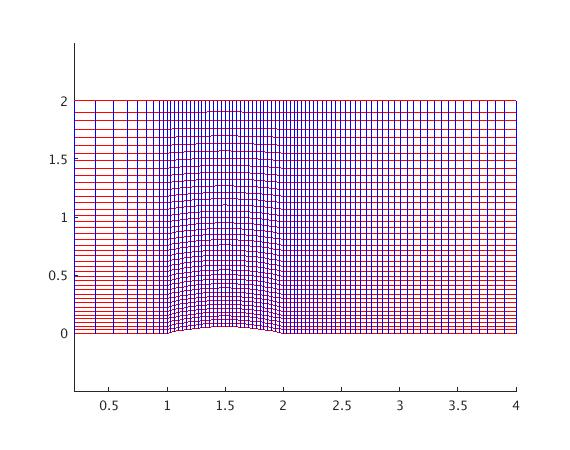
\includegraphics[width= 0.8\textwidth]{Figures/Meshc.jpg} 
\caption[81x41 airfoil mesh]{81x41 airfoil mesh}
\label{fig:mesh}
\end{figure}
\end{lstlisting}

The htbp refers to the placement the figure in order and \LaTeX\ will decide which is best. The htbp refers to: here, top, bottom or next page. \LaTeX\ will do what it finds best the ! is to force it to do what you say and not what it feels is best.

The centering command as you may have guessed is to centre align the figure. The third line is where you actually insert the figure and set the width you would like, in this example the width is 80 \% of the text width. The figure is located in the Figures subdirectory in the same directory as the .tex file.

The caption has two parts the caption in square brackets is what will be displayed in the list of figures and the curly brackets caption will be displayed below the figure. If these two are the same you may simply leave out the square brackets. The label is sort of the variable name for the figure and what would be used to reference the figure in text for eg.: $\backslash$ref\{fig:mesh\}. The label name can be made anything fig, tab and eq are simply used to group the labels for similar objects together to find it easier in the suggestion box when referencing in text.

\begin{figure}[!htbp]
\centering
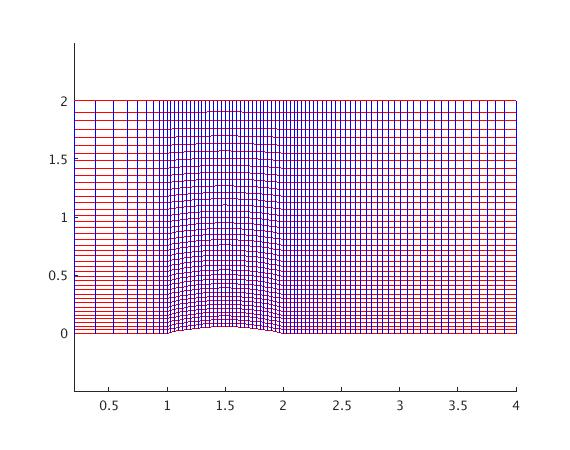
\includegraphics[width= 0.8\textwidth]{Figures/Meshc.jpg}
\caption[81x41 airfoil mesh]{81x41 airfoil mesh}
\label{fig:mesh}
\end{figure}

To insert two figures alongside each other a minipage environment can be used. Two minipages are created in a figure environment with the width of each mini page less than 50 \% of the text width or else the figures will be below each other.

\begin{figure}[!htbp]
\centering
\begin{minipage}[t]{0.48\textwidth} 
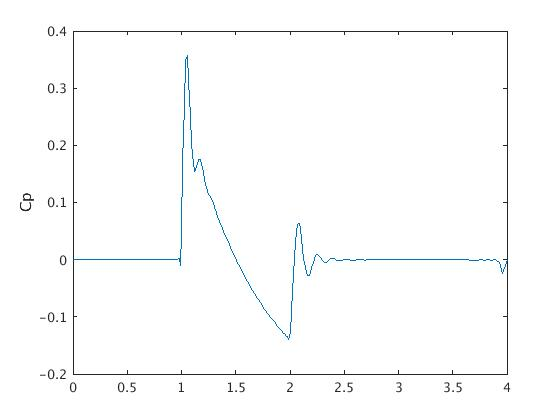
\includegraphics[width= \textwidth]{Figures/cp.jpg}
\caption{Pressure coefficient against airfoil}
\label{fig:cp}
\end{minipage}
\begin{minipage}[t]{0.48\textwidth} 
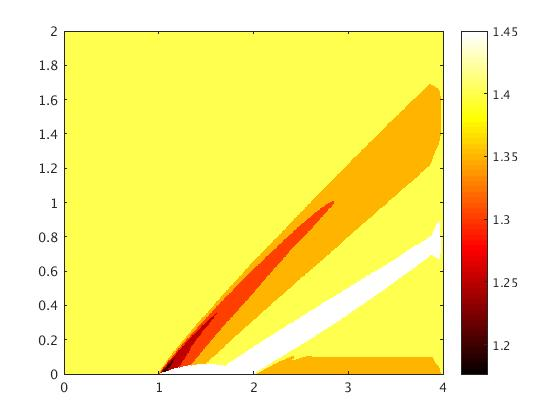
\includegraphics[width= \textwidth]{Figures/machcontour.jpg}
\caption{Contour plot of mach number against the airfoil}
\label{fig:mach}
\end{minipage}
\end{figure}    

\subsection{Mathematics}
The excerpt below is to insert an equation:
\begin{lstlisting}
\begin{equation}
\dfrac{\partial \rho}{\partial t} + \nabla \cdot (\rho \bar{u}) = 0
\label{eq:continuity}
\end{equation}
\end{lstlisting}
For equations Greek symbols can be entered by simply typing the name of the symbol with the first character a capital letter if the upper case Greek symbol is required. Refer to \href{https://www.sharelatex.com/learn/List_of_Greek_letters_and_math_symbols}{www.sharelatex.com} for more information on Greek and mathematical symbols.
\begin{equation}
\label{eq:continuity}
\frac{\partial \rho}{\partial t} + \nabla \cdot (\rho \bar{u}) = 0
\end{equation}
\nomenclature{$\rho$}{Density (\si{\kilo \gram \per \cubic \meter})}
\nomenclature{$t$}{Time (\si{\second})}
\nomenclature{$u$}{Velocity (\si{\meter \per \second})}

\subsection{Tables}
The main structure of the table is similar to that of a figure, once again there is a begin table command, a command to centre the table with a caption and a label only the caption is at the top now according to departmental guidelines. The excerpt below shows how to create a table in \LaTeX\ with the result below in Table \ref{tab:fpiorder}.
\begin{lstlisting}
\begin{table}[!ht]
\centering
\caption{FPI rate and order of convergence}
\label{tab:fpiorder}
\begin{tabular}{lll}
\toprule
k$_s$ & q & $\mu$  \\
\midrule
1 & 0.9940& -0.1761\\
2 & 0.9887 & -0.2896\\
4 & 0.9895& -0.4366\\
\bottomrule
\end{tabular}
\end{table}
\end{lstlisting}
The begin tabular command with {lll} afterwards tells \LaTeX\ to create a table with left aligned columns. The top and bottom thicker lines can be made using the $\backslash$toprule and $\backslash$bottomrule commands. The thinner inside lines can be made by using $\backslash$midrule.


\begin{table}[!ht]
\centering
\caption{FPI rate and order of convergence}
\label{tab:fpiorder}
\begin{tabular}{lll}
\toprule
k$_s$ & q & $\mu$  \\
\midrule
1 & 0.9940& -0.1761\\
2 & 0.9887 & -0.2896\\
4 & 0.9895& -0.4366\\
\bottomrule
\end{tabular}
\end{table}

\subsection{Referencing}
In text referencing to a figure, table or equation is done by simply using the ref command. \LaTeX\ keeps track of the numbering so you don't have to the numbering will stay correct even if you move things around \LaTeX\ knows how to count. Here is an example of how to reference a figure: Table $\backslash$ref\{tab:fpiorder\} shows the order of convergence for fixed point iteration. This example will result in: Table \ref{tab:fpiorder} shows the order of convergence for fixed point iteration.

When referencing literature you need to add your reference to the .bib file. The references in the .bib file can then be used in your report, to reference in text the methods in Table ref can be used.

\begin{table}[!ht]
\centering
\caption{In text literature referencing examples}
\label{tab:Cite}
\begin{tabular}{ll}
\toprule
\LaTeX\ syntax & Result\\
\midrule
$\backslash$parencite\{forster1955\} &\parencite{forster1955} \\
$\backslash$textcite\{forster1955\} & \textcite{forster1955} \\
$\backslash$parencite[250]\{cengel2015\} &\parencite[250]{cengel2015} \\
$\backslash$textcite[250]\{cengel2015\} & \textcite[250]{cengel2015} \\
\bottomrule
\end{tabular}
\end{table}

This will create your reference list correct according to the departmental guidelines. Below is an example of a book and an article reference.
\begin{lstlisting}
@Book{cengel2015,
  author		= {\c{C}engel, Y A and Ghajar, A J},
  title			= {Heat and Mass Transfer},
  publisher		= {McGraw-Hill},
  year			= 2015,
  address		= {New York},
  edition		= 5
}

@Article{forster1955,
  author		= {Forster, K and Zuber, N},
  title			= {Dynamics of vapour bubbles and boiling heat-transfer},
  journal		= {AIChE Jl},
  year		= 1955,
  pages		= {531},
  volume		= {1}
}
\end{lstlisting}

To create your reference list at the end of your document it is as simple as typing: 
\begin{lstlisting}
\printbibliography
\end{lstlisting} 


\printbibliography
\appendix
\renewcommand{\thefigure}{\thesection.\arabic{figure}}
\renewcommand{\thetable}{\thesection.\arabic{table}}
\renewcommand{\thepage}{\thesection.\arabic{page}}
\end{document}